\chapter{GANs and creativity}
\label{ch:generative_or_creative}

% OK

An important, but often difficult to answer, question in the CC field is whether a system is creative or simply generative.
To defend the claim of GANs being capable of becoming creative systems, the main idea behind them is first explained in a simplified manner.
The black box problem of GANs is discussed together with the challenges it forms.
This chapter concludes with a more philosophical take on why GANs can be creative systems.

%------------------------------------
\section{Main idea behind a GAN}
\label{sec:main_idea_GAN}

Figure \ref{fig:gan_explained} shows a visualisation of the different components of a GAN.
It becomes visible that there are two systems at play, a discriminator and a generator.
The discriminator has access to the database containing images of the concept the GAN should generate new instances for.
Its job is to either accept or reject an incoming image.
An image that is accepted can be seen as one that the discriminator finds to be of the concept it has learned and thinks it is not computer-generated.
In some instances, the discriminator is a continuous learning algorithm.
The generator learns by starting from a random noise vector and transforming it until it receives something accepted by the discriminator.
The main differences between different GAN technologies are the way how they implement the generator.


\begin{figure}[H]
    \centering
    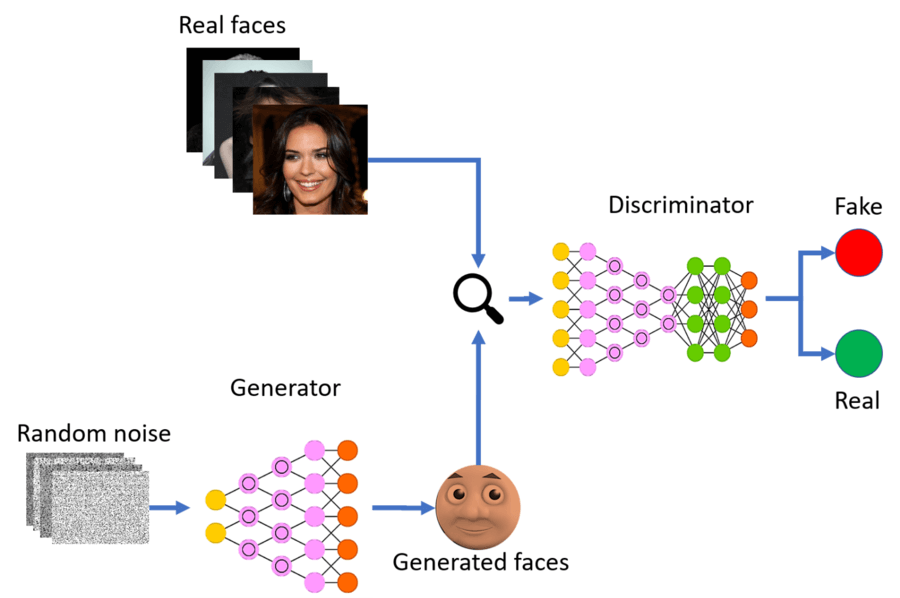
\includegraphics[width=0.55\linewidth]{images/gan_explained.png}
    \captionsetup{width=0.4\linewidth}
    \captionsetup{justification=centering}
    \caption{Basic idea of a GAN. Figure by \citet{howganworks}.  }
    \label{fig:gan_explained}
\end{figure}

%------------------------------------
\section{Black box problem}
\label{sec:back_box_problem}

One issue with GANs is that they almost always make use of deep NNs for both their generator and discriminator.
A deep NN is known to be a black-box model.
This means that there is no meaningful insight on how the model works, it is just a bunch of mathematical manipulations a human cannot reason about.
This makes it hard to state that a deep NN has learned something.
One can only evaluate if the output is what is desired.
This introduces the risk of claiming that you think a deep NN has learned something whilst in reality it might have learned something completely different which happens to give the same desired output by chance.
This is an important issue for AI in general.
An academic example that is often given to demonstrate this point is one where a tank recognition NN didn't learn to differentiate trees and tanks but rather the time of the day, which happened to correspond with the presence of tanks for the training and test samples.
Whilst this example demonstrates the issue at hand, it is noted that it could be an urban legend as discussed in a blog post by Gwern Branwen \footnote{\url{https://www.gwern.net/Tanks}}.


%------------------------------------
\section{GANs as creative systems}
\label{sec:GAN_as_creative}

In the CC field, understanding the process for achieving an output that might be deemed creative by humans is an important manner in deeming a system creative.
This makes algorithms with the black box problem such as GANs a hard case for creative systems.
However, the discussed DARCI system by \citet{darci} shows that systems using NNs can indeed be deemed creative if defended appropriately.
One of the convincing strengths of DARCI is that it gives a natural language description of the steps it takes to generate an image.
These are things such as explaining what image of the training set it relates to and what the labels for that known image are.
These descriptions aim to give an insight into the process of the creative system to try and tackle the black box problem.
However, DARCI does not know the semantic meaning of those descriptions and labels.
All of the natural language descriptions and labels were provided by a human as training data and statistically processed by the system.
It is even very likely that the internal representation of those strings is numerical through encoding.
Knowing this, the natural descriptions it delivers are likely to give the false perception that the system has a sense of semantic reasoning, which it does not.
It also gives a wrong idea of how the generative process of the system works.

Not all is bad though, as is mentioned in the paper on how to build a CC system by \citet{ventura}, some argue that not knowing what aesthetic the system is using is a positive advance as it gives more freedom and thus enhances creativity.
Whilst it would be easy to just agree with this as a defence on why explainability shouldn't be of huge concern for the CC field, there are some issues with this.
First of all, Ventura is a co-author of the older DARCI system.
Since DARCI uses NNs, Ventura couldn't suddenly state explainability are a must for creative systems, as that would render DARCI a non-creative system.
His use of GANs as examples in the paper further shows his stance on this topic.
However, one of the three characteristic Ventura gives to computationally creative agents is intentionality.
To defend intentionality correctly, a certain idea of how the generative process works needs to be present.
Explainability is also something that is desired for scientific fields in general.

\clearpage
So, where does this leave GANs as (part of) a creative system?
As it turns out, the days of true black-box models, where no analysis on learned concepts was performed, seem to have passed.
This is mainly due to new regulations being hard on the explainability of AI algorithms. 
Since deep NNs are often the desired solution for AI problems, much research in making them explainable is being done.

Papers such as the one by \citet{invidualunitanalysis} have an interesting approach to enhance explainability.
They analyse the meaning of individual units of a deep NN by disabling or boosting their output.
From this, they conclude multiple things.
One example is the detection of units that are responsible for generating trees, as disabling them drastically lowers the generation of trees and vice versa.
These approaches are steps in making it more defensible that a deep NN has indeed learned certain concepts.
This leads to why tools such as GANSpace can aid in the explainability of a GAN.
It also gives an insight into the generation process of the GAN and thus the use of GANs in the CC field becomes more viable.
If it is possible to determine components within one or more layers of the GAN to be responsible for the creation of distinct concepts in hundreds of samples, can it then not be claimed the system has learned that concept?
When does luck become skill?
On the GitHub repository for this paper, multiple examples of changing distinct concepts through GANSpace can be found.
Some are also discussed in the evaluation chapter of this paper and shown in figure \ref{fig:groupedsurvey}.
From this, it becomes clear the system does have an explainable generation process that consists of generating multiple distinct concepts to form a final image.

Once the above statements about the GAN's generation procedure are accepted, it's an easier step towards claiming them creative systems.
In the discussed internal working of a GAN, it is visible that internal evaluation is a crucial part of the design already.
GANs are also more than just an optimisation problem, as there is no "best image to generate", much as there is no "best artwork to generate".
Since the generator doesn't have direct access to the dataset and uses random noise vectors as its input it becomes clear it is creating things from the knowledge it has learned through the discriminator.
From the above statements, it becomes clear that knowledge is indeed meaningful concepts rather than random values.
The training loop then limits the conceptual space of the generator from all possible combinations of pixels to all images accepted by the discriminator.
This process corresponds to the generator becoming better at understanding the different concepts a car design requires.

One of the only challenges remaining to deem GANs creative is whether or not the created images are different enough from existing cars.
A reverse image search analysis, such as the ones used by Google reverse image search, can be used to ensure novelty.
Most of such state-of-the-art algorithms for this task also use deep NNs.
A recent paper by \citet{reverseimagesearch} discusses how such behaviour could be reached by using a pre-trained convolutional NN.
It is noted that adding such an evaluation metric would only ensure P-creativity, as it only has access to the training images and not all cars ever made.
It is also important to remember from the domain explanation that similarity to existing models is expected and often even desired in car design.
Thus, for this specific domain, there should possibly even be a lower bound for this similarity metric.
Having hyper-parameters for these thresholds is recommended.
With this final required component of the system in place, it can be seen that GANs can indeed be creative systems.